\documentclass[journal,onecolumn]{IEEEtran}

% include a few useful packages; you will probably want more
\usepackage{graphicx} 
\usepackage[margin=1in]{geometry} 
\usepackage{amsmath,amsthm,amssymb}
\usepackage[noend]{algpseudocode}
\usepackage[hypcap=true]{caption}
\usepackage{lipsum}
\usepackage{float}
\makeatletter
\def\BState{\State\hskip-\ALG@thistlm}
\makeatother
\usepackage{algorithm}
% place all photos and diagrams in the media folder
\graphicspath{{media/}}

\hyphenation{op-tical net-works semi-conduc-tor}

\begin{document}

\title{%
  ROB 550 BotLab Report \\
  %\large Prototype Implementations of SLAM and A* for a Wheeled Robot
  }
    
\author{Saptadeep Debnath - saptadeb@umich.edu}

\maketitle

\IEEEpeerreviewmaketitle

\section{MAPPING AND SLAM}

\subsection*{1.1 - Mapping - Occupancy Grid} 

Write a paragraph or two description including the following:

\begin{itemize}
    \item Provide the values of the incremental log odds you're using for a free \& occupied cells.
    \item Describe the method used determine which cells to update.
    \item Comment on mapping behavior.
\end{itemize}

The mapping function is implemented in two stages - first we score the cells which are located at the endpoint of the rays. If the cells corresponding to the endpoint of the rays are in the given map, log odds for the cell are increased by `3', defining the boundaries. Next, the cells between the robot cell and the endpoint cell are scored. Bresenham's line algorithm is then used to rasterize the given ray. The log odds of these free cells are then decreased by `1'. 

The maps generated when the robot is stationary as is in the case of convex\_grid\_10mx10m\_5cm.log are not quite accurate at far away points. As the robot is stationary the laser rays originating from that position diverge farther away from each other at long distances, because of which some of the cells in between those rays don't get scored. This problem is mitigated when the robot is in motion; wherein because of the motion of the robot the laser rays tend to cover most of the grid cells and hence we obtain a better map in the end.  

\subsection*{1.2.1 - MCL - Action Model} 

 Write a paragraph or two description including the following:
 \begin{itemize}
    \item Specify what type of action model you're using.
    \item Provide all noise constants that you're using.
    \item Comment on the your action model:
        \begin{itemize}
            \item Does the distribution grow as expected for the particles?
            \item Do you think the action model constants will differ drastically from one
mbot to another?
        \end{itemize}
\end{itemize}

Out of the two most widely used motion models, odometry motion model is used over the velocity motion model for this project. Odometry information is obtained by integrating the wheel encoder information over periodic time intervals. It is however observed that even though the odometry action model isn't perfect, it provides a better approximation of the robot motion than the velocity model for predicting the robot motion.

In order to predict the robot pose the odometry information (i.e. x, y and $\theta$) is changed to an RTR information given by equation \ref{eq:RTR}, i.e rotation-translate-rotation which is sampled with a Gaussian noise distribution in the form described in equation \ref{eq:fullRTR}. In the initial phases of the project the values of the noise constants were chosen as $k_1 = 0.8$ and $k_2 = 0.3$. On further inspection and to reduce the computation load to calculate the standard deviation for each odometry information, the standard deviations are given as constants, where ${\sigma}^2_{rot1} = 0.05$, ${\sigma}^2_{trans} = 0.005$ and ${\sigma}^2_{rot2} = 0.05$. These noise constants are chosen and tuned in order to achieve a better spread of distribution of the particles and to achieve a more accurate proposal which is used for the sensor model. It is expected to see the tuning parameters differ from one mbot to another, but the difference should be small as the make and model of the mbot is consistent The elements which could factor into a possible drastic difference between the tuning parameters from one mbot to another could be the systematic errors related to the specific mbot.

\begin{equation}\label{eq:RTR}
\begin{split}
	\delta_{rot1} &= atan2(y_t - y_{t-1}, x_t - x_{t-1}) - \theta_{t-1}	\\
	\delta_{trans} &= \sqrt{(x_t - x_{t-1})^2 - 	(y_t - y_{t-1})^2}	\\
	\delta_{rot2} &= \theta_t - \theta_{t-1} - \delta_{rot1}
\end{split}
\end{equation}

\begin{equation}\label{eq:fullRTR}
\begin{split}
	\hat{\delta}_{rot1} & \sim \mathcal{N}(\delta_{rot1},\,k_1 \cdot \mid\delta_{rot1}\mid)	\\
	\hat{\delta}_{trans} &\sim \mathcal{N}(\delta_{trans},\,k_2 \cdot \mid\delta_{trans}\mid)	\\
	\hat{\delta}_{rot2} &\sim \mathcal{N}(\delta_{rot2},\,k_1 \cdot \mid\delta_{rot2}\mid)
\end{split}
\end{equation}

\begin{figure}[H]
\centering
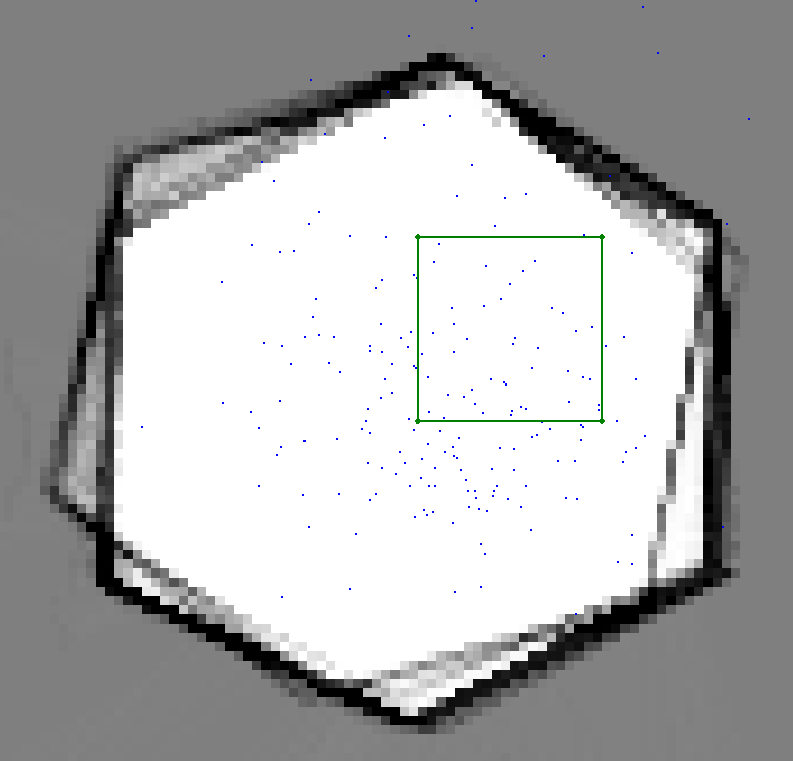
\includegraphics[width=0.3\textwidth]{Media/1211.png}
\caption{Particle distribution obtained at the end of drive square with action only}
\end{figure}

\begin{figure}[H]
\centering
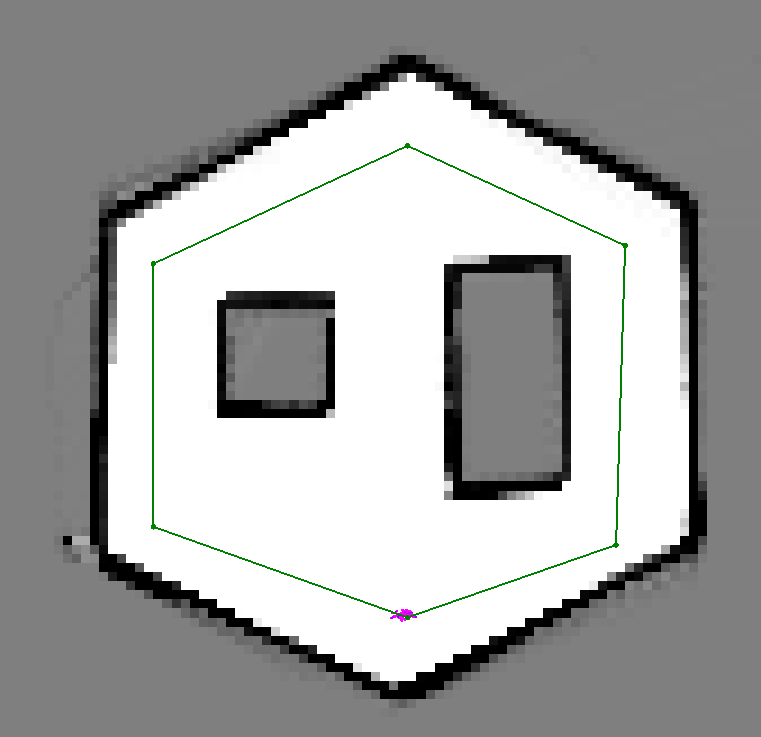
\includegraphics[width=0.3\textwidth]{Media/1212.png}
\caption{Particle distribution obtained at the end of obstacle slam with action only}
\end{figure}

\begin{figure}[H]
\centering
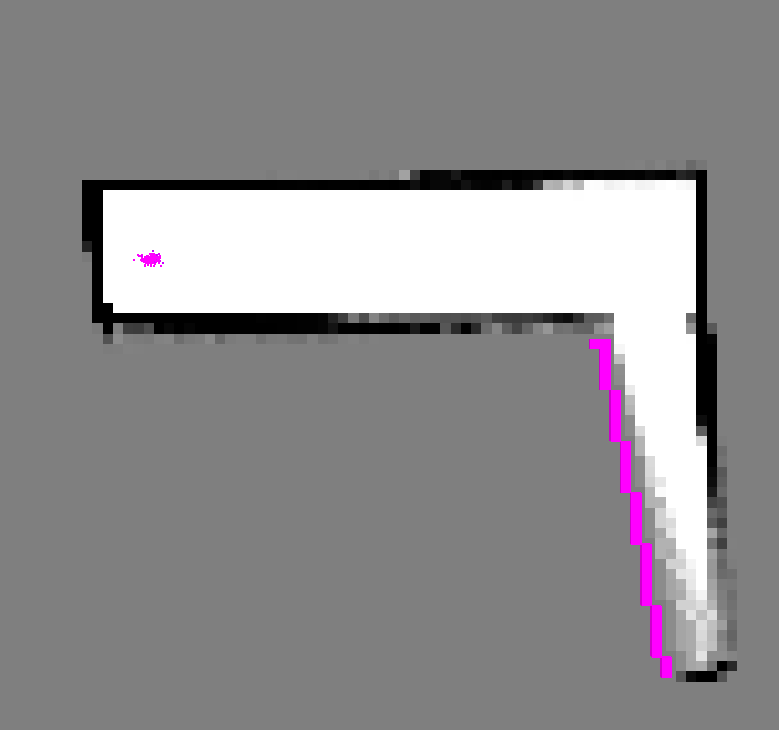
\includegraphics[width=0.3\textwidth]{Media/1213.png}
\caption{Particle distribution obtained at the end of straight line calm with action only}
\end{figure}

\subsection*{1.2.2 - MCL - Sensor Model \& Particle Filter} 

 Write a paragraph or two description including the following:
 \begin{itemize}
    \item Specify what type of sensor model you're using, and how you are weighting and resampling.
    \item Provide all noise constants that you're using.
    \item Is the estimated pose closer to the true pose with your localized pose estimate compared to that from odometry?
    \item Do the particles remain in a tight region as the robot moves?
    \item Do the particles spread more aggressively with a certain motion type? (rotation, for example).
\end{itemize}

\begin{figure}[H]
\centering
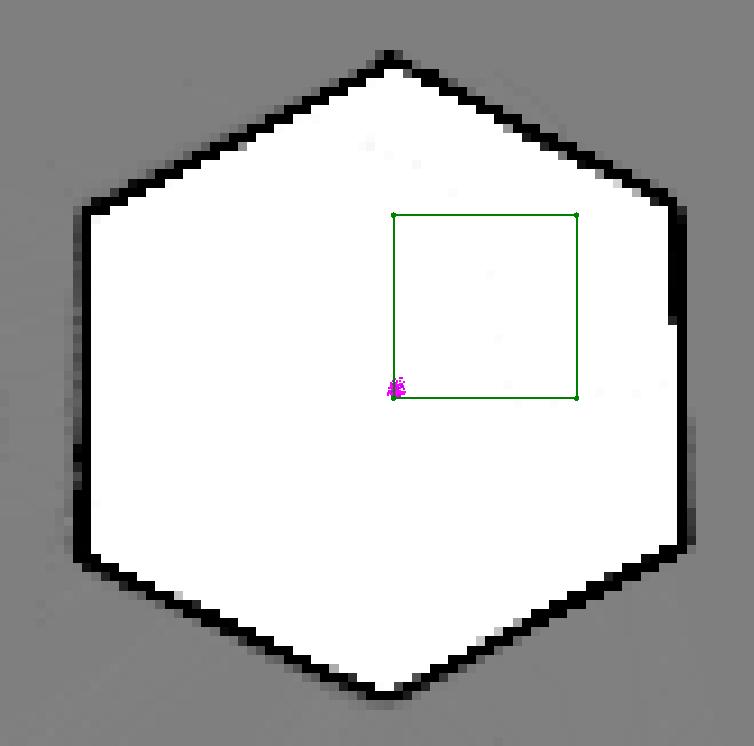
\includegraphics[width=0.3\textwidth]{Media/1221.png}
\caption{Particle distribution obtained at the end of drive square with localization only}
\end{figure}

\begin{figure}[H]
\centering
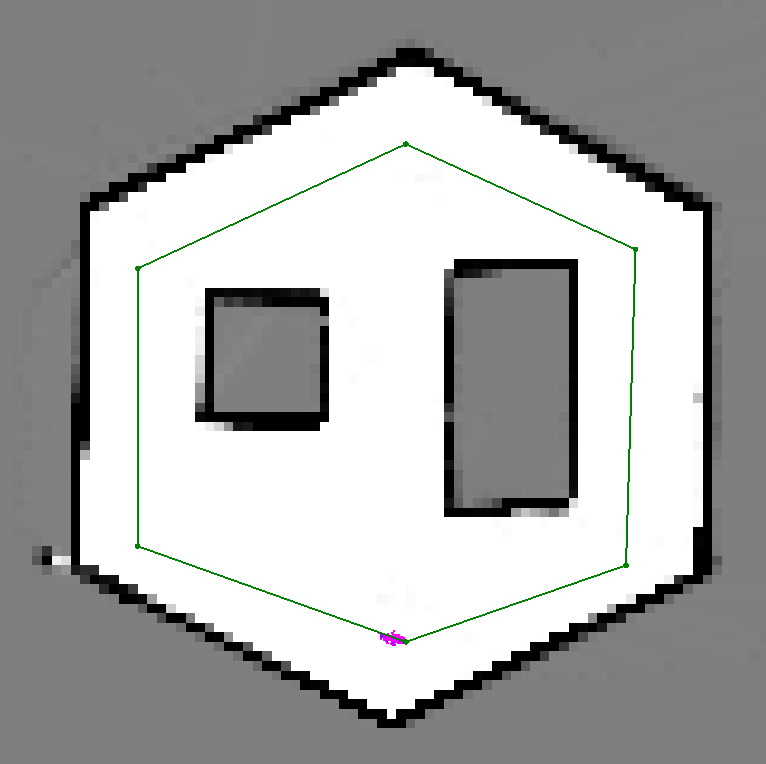
\includegraphics[width=0.3\textwidth]{Media/1222.png}
\caption{Particle distribution obtained at the end of obstacle slam with localization only}
\end{figure}


\begin{figure}[H]
\centering
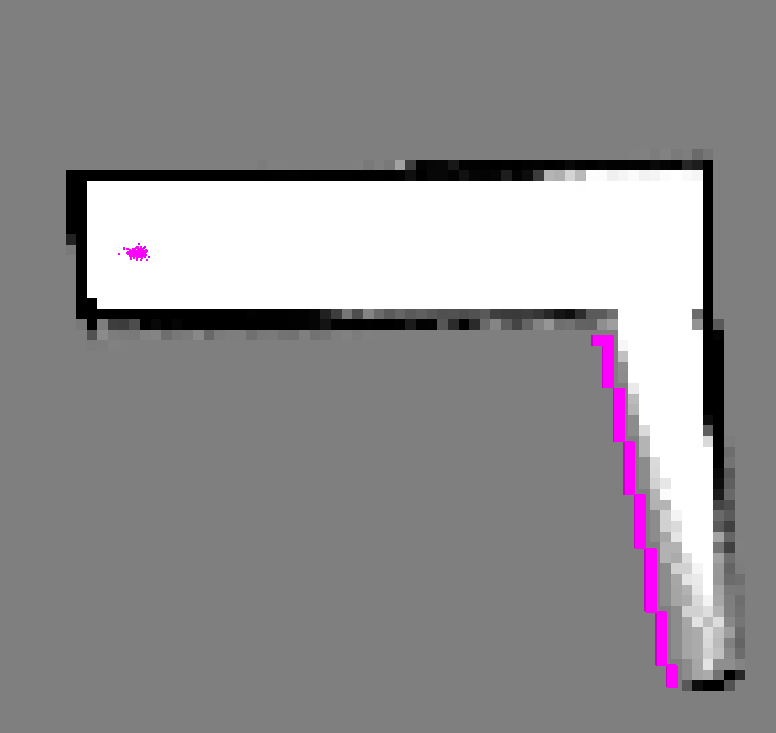
\includegraphics[width=0.3\textwidth]{Media/1223.png}
\caption{Particle distribution obtained at the end of straight line with localization only}
\end{figure}

\subsection*{1.3 - Simultaneous Localization and Mapping (SLAM)} 

 Write a paragraph or two description including the following:
 \begin{itemize}
    \item Did you obtain similar/close performance for obstacle\_slam\_10mx10m\_5cm.log compared to the previous two runs? Why or why not?
    \item Did the change of map resolution affect your computation time? Did it improve/harm your slam results?
    \item Did you have to change your mapping log odds to improve on performance? If so, report them.
\end{itemize}

\begin{figure}[H]
\centering
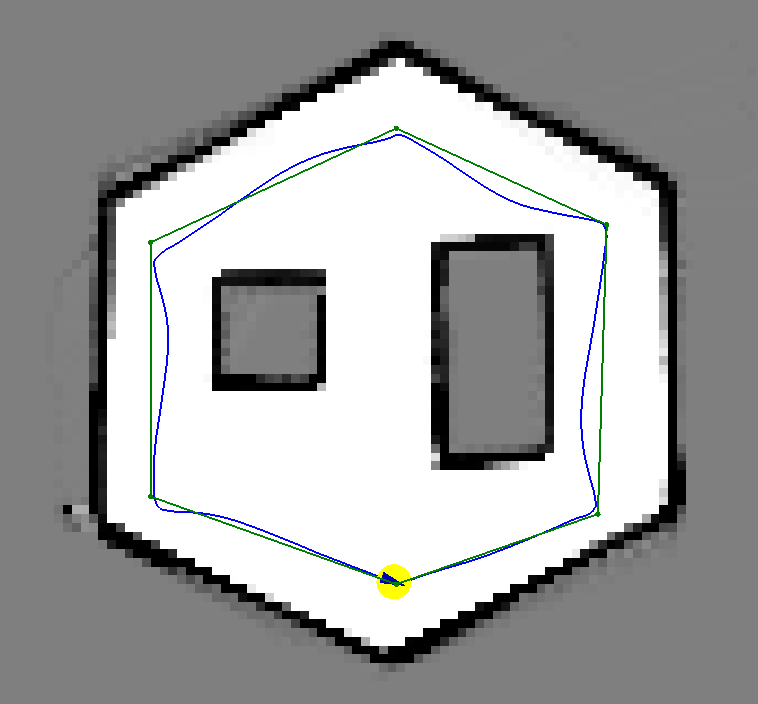
\includegraphics[width=0.3\textwidth]{Media/131.png}
\caption{Particle distribution obtained at the end of Obstacle Slam with Full SLAM}
\end{figure}

\begin{figure}[H]
\centering

\includegraphics[width=0.3\textwidth]{Media/template-robotics.jpg}
\caption{Particle distribution obtained at the end of Maze LowRes with Full SLAM}
\end{figure}

\begin{figure}[H]
\centering

\includegraphics[width=0.3\textwidth]{Media/template-robotics.jpg}
\caption{Particle distribution obtained at the end of Maze HiRes with Full SLAM}
\end{figure}

\begin{figure}[H]
\centering

\includegraphics[width=0.3\textwidth]{Media/template-robotics.jpg}
\caption{Particle distribution obtained at the end of Maze Hard with Full SLAM}
\end{figure}

\section{PATH PLANNING AND EXPLORATION}

\subsection*{2.1 - Obstacle Distances} 

Comment on whether your code passed or failed the three tests in obstacle\_distance\_grid\_test. Provide remarks on the code’s performance and whether there is anything major slowing it down.

\begin{figure}[H]
\centering
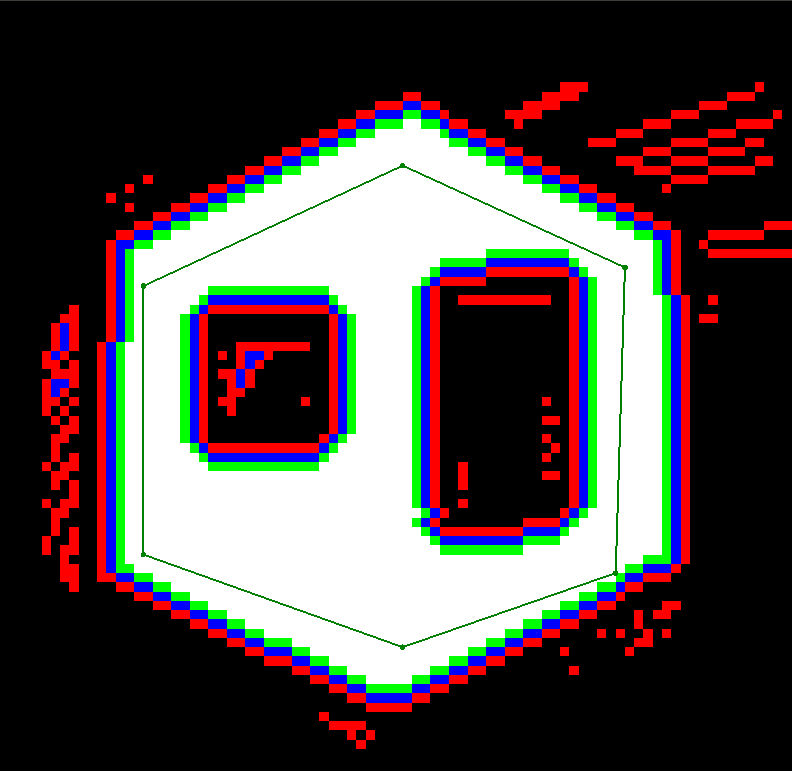
\includegraphics[width=0.3\textwidth]{Media/21.png}
\caption{Obstacle distance grip obtained at the end of Obstacle Slam with Full SLAM}
\end{figure}


\subsection*{2.2 - A* Path Planning} 

Report statistics on your path planning execution times for each of the example problems in the data/astar folder. If your algorithm is optimal and fast, great. If not please discuss possible reasons and strategies for improvement.

\begin{figure}[H]
\centering

\includegraphics[width=0.3\textwidth]{Media/template-robotics.jpg}
\caption{Path obtained at the end of Maze HiRes with A* path planning}
\end{figure}

\subsection*{2.3 - Map Exploration} 

Comment on your exploration performance:
 \begin{itemize}
    \item What are the factors that are preventing your exploration from being ideal?
    \item Provide your logic behind tackling frontiers (how do you go about chosing your next frontier to go to)
    \item Comments on the performance of Astar and path planning with automated exploration commands.
\end{itemize}

\ifCLASSOPTIONcaptionsoff
  \newpage
\fi

% Include your citations in the references.bib file
\nocite{*}
\bibliographystyle{IEEEtran}
\bibliography{references.bib}
\end{document}